\chapter{Project Plan}

\section{Project Implementation Plan}
The implementation trajectory of StepCharge AI is structured across distinct engineering phases corresponding to the academic milestones of the Bachelor of Engineering curriculum. Table~\ref{tab:implementation_plan} delineates the task schedule, duration, and completion statuses.

\begin{table}[H]
\centering
\small
\renewcommand{\arraystretch}{1.2}
\caption{System implementation plan and milestone schedule.}
\label{tab:implementation_plan}
\begin{tabular}{|c|p{2.3in}|c|c|c|}
\hline
\textbf{Sr. No.} & \textbf{Task Description} & \textbf{Start Date} & \textbf{End Date} & \textbf{Status} \\
\hline
1 & Project Ideation \& Problem Formulation & 01/07/2026 & 15/07/2026 & Completed \\
\hline
2 & Comprehensive Literature Survey & 16/07/2026 & 31/07/2026 & Completed \\
\hline
3 & SRS Preparation \& Requirement Analysis & 01/08/2026 & 14/08/2026 & Completed \\
\hline
4 & Feasibility Study \& Component Sourcing & 15/08/2026 & 31/08/2026 & Completed \\
\hline
5 & Hardware Circuit Design \& Prototyping & 01/09/2026 & 25/09/2026 & Completed \\
\hline
6 & ESP32 Firmware Development \& Calibration & 26/09/2026 & 15/10/2026 & Completed \\
\hline
7 & Backend API \& Database Pipeline & 16/10/2026 & 05/11/2026 & Completed \\
\hline
8 & Machine Learning Model Training \& Evaluation & 06/11/2026 & 20/11/2026 & Completed \\
\hline
9 & React Web Dashboard Implementation & 21/11/2026 & 10/12/2026 & Completed \\
\hline
10 & Preliminary Project Report \& Presentation & 11/12/2026 & 30/12/2026 & Ongoing \\
\hline
11 & Multi-Tile Expansion \& TinyML Optimization & 05/01/2027 & 28/02/2027 & Planned \\
\hline
12 & Final Testing, Field Trials \& Project Defense & 01/03/2027 & 31/03/2027 & Planned \\
\hline
\end{tabular}
\end{table}

\section{Work Breakdown Structure (WBS)}
The project is organized hierarchically into five primary work packages:
\begin{enumerate}
    \item \textbf{1.0 Hardware and Mechanical Engineering:}
    \begin{itemize}
        \item 1.1 Piezoelectric transducer selection and impedance testing.
        \item 1.2 Tile mechanical housing and elastomeric suspension fabrication.
        \item 1.3 Schottky rectification, Zener clamping, and supercapacitor circuit assembly.
        \item 1.4 Precision resistive divider calibration.
    \end{itemize}
    \item \textbf{2.0 Embedded Firmware Engineering:}
    \begin{itemize}
        \item 2.1 ESP32 analog sampling and 16$\times$ oversampling configuration.
        \item 2.2 Digital filtering and Exponential Moving Average (EMA) smoothing.
        \item 2.3 Dual-threshold Schmitt trigger hysteresis implementation.
        \item 2.4 Refractory lockout and pulse duration filtering routines.
        \item 2.5 HTTPS client and JSON serialization pipeline.
    \end{itemize}
    \item \textbf{3.0 Cloud Backend and Database Engineering:}
    \begin{itemize}
        \item 3.1 Node.js and Express RESTful API gateway development.
        \item 3.2 SHA-256 cryptographic device key authentication middleware.
        \item 3.3 Google OAuth 2.0 and HttpOnly session management.
        \item 3.4 MongoDB Atlas schema modeling and compound time-series indexing.
        \item 3.5 Socket.IO room subscription and real-time event broadcasting.
    \end{itemize}
    \item \textbf{4.0 Machine Learning Microservice:}
    \begin{itemize}
        \item 4.1 Ground-truth dataset collection and physical boundary verification.
        \item 4.2 Time-domain kinetic feature extraction.
        \item 4.3 Random Forest classifier training with GroupKFold cross-validation.
        \item 4.4 High-throughput FastAPI HTTP inference microservice.
    \end{itemize}
    \item \textbf{5.0 Web Dashboard and Presentation Client:}
    \begin{itemize}
        \item 5.1 React 19 component hierarchy and Tailwind CSS styling.
        \item 5.2 Real-time SVG dials and time-series charting.
        \item 5.3 Closed-loop MOSFET load actuation toggles.
        \item 5.4 Accessible user profile and notification drawer interfaces.
    \end{itemize}
\end{enumerate}

\section{Gantt Chart}
Figure~\ref{fig:gantt_chart} illustrates the project execution timeline across Semester 1 and Semester 2 of the 2026--27 academic year.

\begin{figure}[H]
\centering
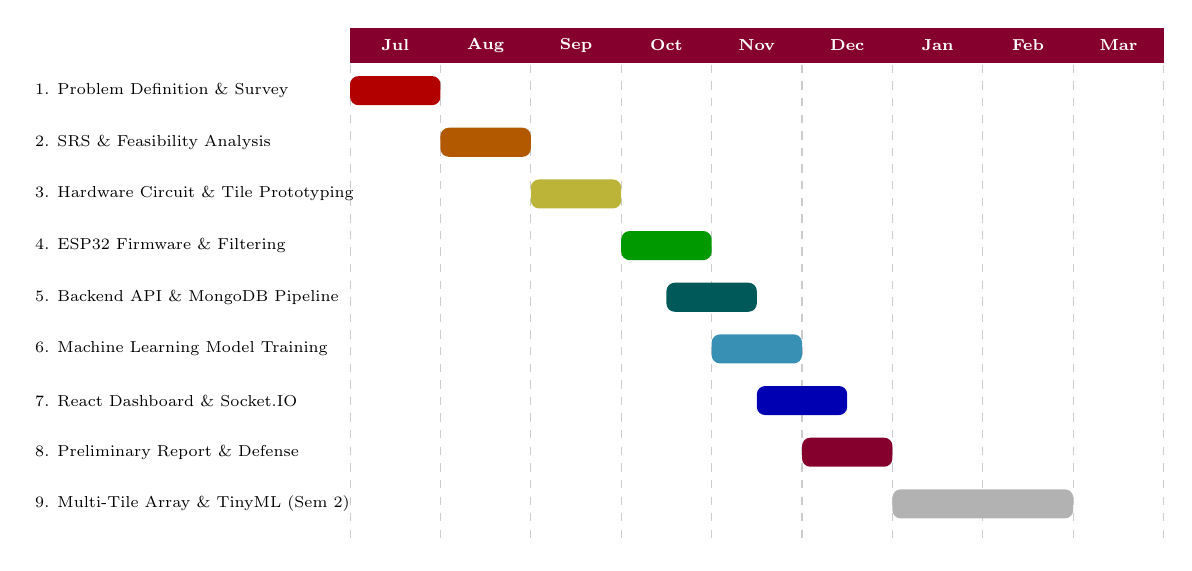
\begin{tikzpicture}[
    scale=0.82, every node/.style={scale=0.82},
    bar/.style={rectangle, rounded corners=3pt, fill=blue!70!black, minimum height=0.45cm},
    header/.style={rectangle, fill=purple!70!black, text=white, font=\bfseries\scriptsize, minimum height=0.55cm, align=center},
    task/.style={font=\scriptsize, anchor=west}
]
    % Months Header
    \node (m1) [header, minimum width=1.4cm] at (0.7, 7.5) {Jul};
    \node (m2) [header, minimum width=1.4cm] at (2.1, 7.5) {Aug};
    \node (m3) [header, minimum width=1.4cm] at (3.5, 7.5) {Sep};
    \node (m4) [header, minimum width=1.4cm] at (4.9, 7.5) {Oct};
    \node (m5) [header, minimum width=1.4cm] at (6.3, 7.5) {Nov};
    \node (m6) [header, minimum width=1.4cm] at (7.7, 7.5) {Dec};
    \node (m7) [header, minimum width=1.4cm] at (9.1, 7.5) {Jan};
    \node (m8) [header, minimum width=1.4cm] at (10.5, 7.5) {Feb};
    \node (m9) [header, minimum width=1.4cm] at (11.9, 7.5) {Mar};

    % Vertical Grid lines
    \foreach \x in {0.0, 1.4, 2.8, 4.2, 5.6, 7.0, 8.4, 9.8, 11.2, 12.6}
        \draw [dashed, gray!40] (\x, 7.2) -- (\x, -0.2);

    % Tasks and Bars
    \node at (-5.0, 6.8) [task] {1. Problem Definition \& Survey};
    \node at (0.7, 6.8) [bar, fill=red!70!black, minimum width=1.4cm] {};

    \node at (-5.0, 6.0) [task] {2. SRS \& Feasibility Analysis};
    \node at (2.1, 6.0) [bar, fill=orange!70!black, minimum width=1.4cm] {};

    \node at (-5.0, 5.2) [task] {3. Hardware Circuit \& Tile Prototyping};
    \node at (3.5, 5.2) [bar, fill=yellow!70!black, minimum width=1.4cm] {};

    \node at (-5.0, 4.4) [task] {4. ESP32 Firmware \& Filtering};
    \node at (4.9, 4.4) [bar, fill=green!60!black, minimum width=1.4cm] {};

    \node at (-5.0, 3.6) [task] {5. Backend API \& MongoDB Pipeline};
    \node at (5.6, 3.6) [bar, fill=teal!70!black, minimum width=1.4cm] {};

    \node at (-5.0, 2.8) [task] {6. Machine Learning Model Training};
    \node at (6.3, 2.8) [bar, fill=cyan!70!black, minimum width=1.4cm] {};

    \node at (-5.0, 2.0) [task] {7. React Dashboard \& Socket.IO};
    \node at (7.0, 2.0) [bar, fill=blue!70!black, minimum width=1.4cm] {};

    \node at (-5.0, 1.2) [task] {8. Preliminary Report \& Defense};
    \node at (7.7, 1.2) [bar, fill=purple!70!black, minimum width=1.4cm] {};

    \node at (-5.0, 0.4) [task] {9. Multi-Tile Array \& TinyML (Sem 2)};
    \node at (9.8, 0.4) [bar, fill=gray!60, minimum width=2.8cm] {};

\end{tikzpicture}
\caption{Gantt chart illustrating project development phases across Academic Year 2026--27.}
\label{fig:gantt_chart}
\end{figure}

\section{Semester-Wise Activities}
\begin{itemize}
    \item \textbf{Semester 1 Activities (Completed / In Progress):}
    \begin{itemize}
        \item Comprehensive literature survey and review paper formulation.
        \item Formalizing system requirements and drafting the SRS document.
        \item Fabricating the physical 8-transducer piezoelectric tile module.
        \item Implementing the full-wave Schottky bridge and 0.1\,F supercapacitor storage stage.
        \item Coding ESP32 firmware with Schmitt trigger hysteresis and refractory timing.
        \item Engineering the Node.js REST API with SHA-256 device authentication and Google OAuth 2.0.
        \item Persisting time-series telemetry in MongoDB Atlas and streaming via Socket.IO.
        \item Training the initial Random Forest gait classifier via GroupKFold cross-validation.
        \item Developing the React 19 web dashboard and verifying 101 backend unit tests.
        \item Preliminary project report compilation and examination defense.
    \end{itemize}
    \item \textbf{Semester 2 Activities (Planned):}
    \begin{itemize}
        \item Designing an interconnected 4-tile modular walkway array.
        \item Integrating an INA219 current shunt sensor for direct power and current provenance.
        \item Quantizing the classifier for on-device edge execution using TensorFlow Lite Micro.
        \item Extended stress-testing under continuous pedestrian traffic in college corridors.
        \item Final project report, research paper publication, and university oral defense.
    \end{itemize}
\end{itemize}

\section{Work Completed}
All deliverables slated for Semester 1 have been successfully realized, validated by working hardware-in-the-loop tests, automated test suites (101/101 tests passed), and a live web dashboard.

\section{Pending Work}
Pending work reserved for Semester 2 includes multi-tile physical interconnection, on-device TinyML edge inferencing on the ESP32, and long-term environmental fatigue characterization.
